%!TEX root = main.tex
In this section, we are interested in investigating how to transfer knowledge between different agents.

Specifically, we want to see how two agents from different types of networks (one is Value-based network, the other is Policy-based network) can help each other.
% 
Given the dueling Q-network and policy gradient network, we are interested in using Policy gradient network to guide the Dueling Q-network.

\subsection{Knowledge Distillation}


To address this problem, we use Knowledge Distillation \cite{hinton2015distilling} technique to implement our algorithm.

The central idea of using Knowledge Distillation here is to train a network (i.e., dueling Q-network) that partially imitates the outputs of policy gradient network.

In \cite{hinton2015distilling}, this framework is applied to object recognition where the outputs of both teacher and student networks are softmax outputs $P_{t} = softmax(\textbf{a}^{L}_{t})$ and  $P_{s} = softmax(\textbf{a}^{L}_{s})$ 
\begin{equation}
P^{\tau}_{t} = softmax(\frac{\textbf{a}^{L}_{t}}{\tau} )
\end{equation}

\begin{equation}
P^{\tau}_{s} = softmax(\frac{\textbf{a}^{L}_{s}}{\tau} )
\end{equation}
%
where $\textbf{a}^{L}$ is the activation of the last layer $L$ and $\tau > 1$ is the relaxation to soften the outputs of both teacher and student networks. 
%
To relax the outputs of policy network, $\tau >1$ is introduced in the outputs:

Based on the softmax outputs, the student network is trained to optimize the following loss function:
\begin{equation}
\mathcal{L} = \mathcal{H} ( \textbf{y},P_{s} ) + \lambda\mathcal{H} ( P^{\tau}_{t},P^{\tau}_{s} ) 
\end{equation}
where $\mathcal{H}$ is cross-entropy and $\textbf{y}$ is one hot vector of true label. $\lambda$ controls how much knowledge should be transferred from teacher. 
 
\subsection{Guidance on Q-value}

%
We want to investigate whether two totally different networks have complementary information and can guide the other.
%
In our project, the teacher network is the policy gradient network. The student network is the dueling Q-network. The reason that we use policy gradient network to guide dueling Q-network is that policy gradient network performs better than dueling Q-network in our experiments.
%
So, we define our loss function as:
\begin{equation}
\label{equ.kd}
\mathcal{L} = \mathbb{E}(r+\gamma \max_{a'}Q(s',a';\theta^{target}_{Q})-Q(s,a;\theta_{Q})))^2  + \lambda\mathcal{H} ( P^{\tau}_{policy},P^{\tau}_{Q} )
\end{equation}

\noindent
where 
$$P^{\tau}_{policy} = softmax(\frac{\pi(a_i|s_t;\theta_{policy})}{\tau})$$
and  
$$P^{\tau}_{Q} = softmax( \frac{Q(s,a;\theta_{Q})} {\tau} )$$.

\noindent
Specifically, $\pi(a_i|s_t;\theta_{policy})$ is the last layer logits of two networks respectively. To relax the outputs, $\tau$ is set to be 5. $\lambda$ is set te be $0.05$ to balance the loss.

The idea behind Equation \ref{equ.kd} is that the optimal policy at any state usually lead to higher Q-values. Thus we want to use the $\pi(a_i|s_t;\theta_{policy})$ to guide $Q(s,a;\theta_{Q})$.

\subsection{Guidance on mapping of Q-value}
However,  $\pi(a_i|s_t;\theta_{policy})$ is different from $Q(s,a;\theta_{Q})$ semantically. Thus we also proposed another knowledge distillation method: imposing guidance on the mappings.
%
Specifically, we add a fully-connected layer to $Q(s,a;\theta_{Q})$ and obtain  $a^{L+1}_{Q}$.

So now the loss function becomes:
\begin{equation}
\label{equ.kd}
\mathcal{L} = \mathbb{E}(r+\gamma \max_{a'}Q(s',a';\theta^{target}_{Q})-Q(s,a;\theta_{Q})))^2  + \lambda\mathcal{H} ( P^{\tau}_{policy},P^{\tau}_{Q} )
\end{equation}

\noindent
where 
$$P^{\tau}_{policy} = softmax(\frac{\pi(a_i|s_t;\theta_{policy})}{\tau})$$
and  
$$P^{\tau}_{Q} = softmax( \frac{a^{L+1}_{Q}} {\tau} )$$.

Other hyperparameters remain the same.

%
We use a pre-trained policy gradient network which achieves about $3.0$reward to guide the dueling Q-network.


\subsection{Experiment Results}

In this experiment, we compare vanilla dueling Q-network, dueling Q-network guided on Q-values and dueling network guided on mapping of Q-values.

The result is shown in Fig.\ref{fig:mimic_result}. As we can see, the original(vanilla) dueling Q-network performs the best, which means the policy gradient network fails to guide the dueling Q-network.
%
However, as shown in the results, dueling network guided on mapping of Q-values performs better than dueling Q-network guided on Q-values. It means that even though $Q(s,a;\theta_{Q})$ is different from $\pi(a_i|s_t;\theta_{policy})$, we can still project $Q(s,a;\theta_{Q})$ into another space where knowledge can be transfered from $\pi(a_i|s_t;\theta_{policy})$.
\begin{figure}[h!]
	\centering
	\begin{tabular}{c}
		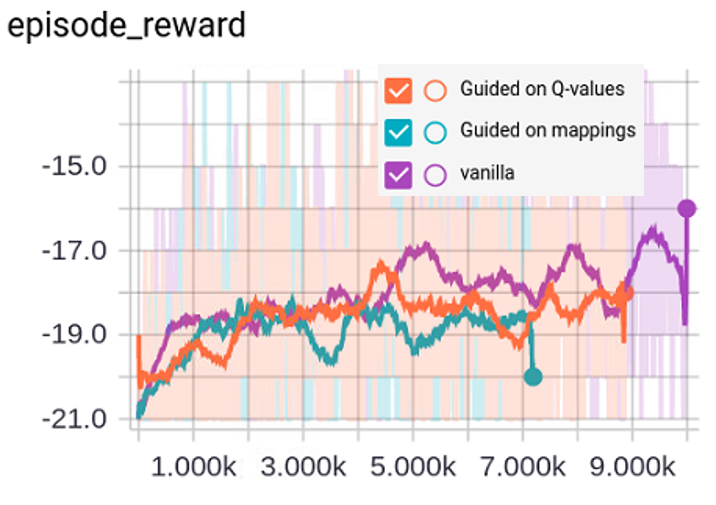
\includegraphics[width=0.49\textwidth]{./fig/mimic_result_episode.png} \\
		(a) Episode reward \\
		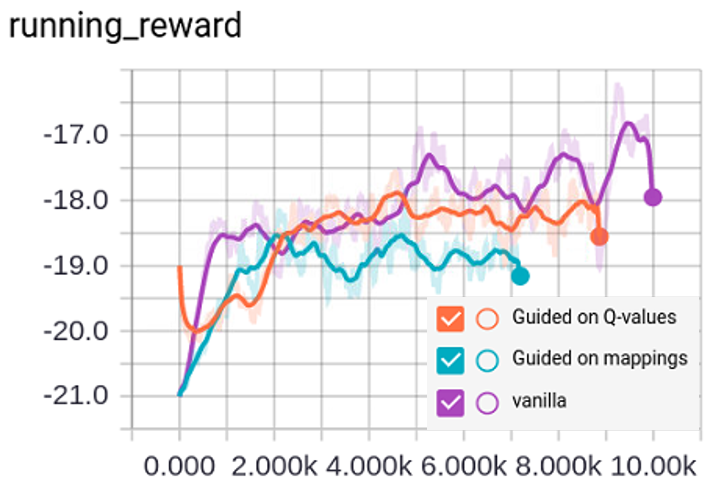
\includegraphics[width=0.49\textwidth]{./fig/mimic_result_running.png} \\
		(b) Running reward \\
	\end{tabular}
	\caption{The rewards of 10K epsiodes on three approaches: vanilla dueling Q-network, dueling Q-network guided on Q-values and dueling network guided on mapping of Q-values. Running reward is the smoothed accumulating rewards}
	\label{fig:mimic_result}
\end{figure}



